\section{Instruction Set}\label{sec:instruction-set}
\pagebreak
\subsection{Load Accumulator}\label{subsec:lda}
    \subsubsection{Syntax}
    \begin{verbatim}lda.[addressing mode]   [8-bit immediate] \end{verbatim}
    \subsubsection{Description}
    $Accumulator \leftarrow OperandValue$
    \par Load the value operand value into the Accumulator.

    \subsubsection{Encoding}
    \begin{center}
        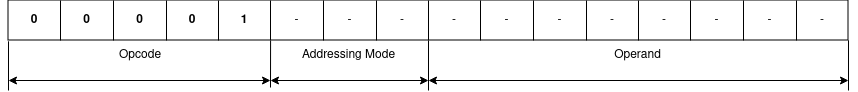
\includegraphics[scale=0.40]{img/Andromeda-LDA.drawio}
    \end{center}

    \subsubsection{Example}
    \begin{verbatim}
        org(0x0000)
    def entry:
        lda.dir     data

        org(0xFF01)
    def data:
        dw(-11)
    \end{verbatim}
    \par The above code would result in `-11' being loaded into the Accumulator.

\pagebreak
\subsection{Store Accumulator}\label{subsec:sta}
    \subsubsection{Description}
    $Memory[AddressOf(OperandValue)] \leftarrow Accumulator $ \\
    \par Store the contents of the accumulator into the address of the operand value.

    \subsubsection{Encoding}
    \begin{center}
        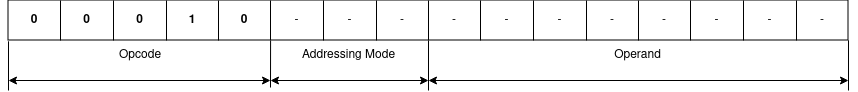
\includegraphics[scale=0.40]{img/Andromeda-STA.drawio}
    \end{center}

    \subsubsection{Example}
    \begin{verbatim}
        org(0x0000)
    def entry:
        lda.imm     -1
        sta.dir     0x01
    \end{verbatim}
    \par The code above would result in `-1' being stored into address 0xFF01.

\pagebreak
\subsection{Add}\label{subsec:add}
    \subsubsection{Syntax}
    \begin{verbatim}add.[addressing mode]   [8-bit immediate]\end{verbatim}

    \subsubsection{Description}
    $Accumulator \leftarrow Accumulator + OperandValue$
    \par Add the operand value to the contents of the Accumulator.
    Store the result in the Accumulator.

    \subsubsection{Encoding}
    \begin{center}
        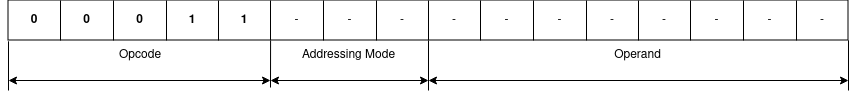
\includegraphics[scale=0.40]{img/Andromeda-ADD.drawio}
    \end{center}

    \subsubsection{Example}
    \begin{verbatim}
        org(0x0000)
    def entry:
        lda.imm     2
        add.imm     2
        hlt
    \end{verbatim}
    \par The above code would result in the number `4' being stored in the Accumulator.

\pagebreak
\subsection{Subtract}\label{subsec:sub}
    \subsubsection{Syntax}
    \begin{verbatim}sub.[addressing mode]   [8-bit immediate]\end{verbatim}

    \subsubsection{Description}
    $Accumulator \leftarrow Accumulator - OperandValue$
    \par Subtract the operand value from the contents of the accumulator.
    Store the result in the Accumulator.

    \subsubsection{Encoding}
    \begin{center}
        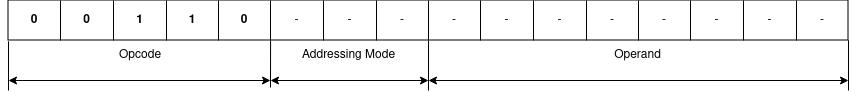
\includegraphics[scale=0.40]{img/Andromeda-SUB.drawio}
    \end{center}

    \subsubsection{Example}
    \begin{verbatim}
        org(0x0000)
    def entry:
        lda.imm     2
        sub.imm     2
        hlt
    \end{verbatim}
    \par The above code would result in a `0' in the Accumulator.

\pagebreak
\subsection{Exclusive Bitwise Or}\label{subsec:xor}
    \subsubsection{Syntax}
    \begin{verbatim}xor.[addressing mode]   [8-bit immediate]\end{verbatim}

    \subsubsection{Description}
    $Accumulator \leftarrow Accumulator \oplus OperandValue$
    \par Bitwise XOR the operand value and the Accumulator.
    Store the result in the Accumulator.

    \subsubsection{Encoding}
    \begin{center}
        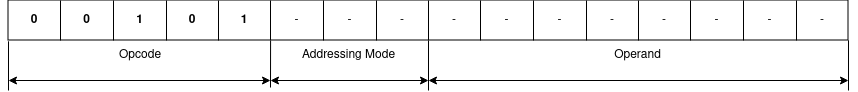
\includegraphics[scale=0.40]{img/Andromeda-XOR.drawio}
    \end{center}

    \subsubsection{Example}
    \begin{verbatim}
        org(0x0000)
    def entry:
        lda.imm     0b00001101
        xor.imm     0b00101110
        hlt
    \end{verbatim}
    \par The code above would result in $00100010_{2}$ being stored into the Accumulator.

\pagebreak
\subsection{Inverted Bitwise And}\label{subsec:nand}
    \subsubsection{Syntax}
    \begin{verbatim}nnd.[addressing mode]   [8-bit immediate] \end{verbatim}

    \subsubsection{Description}
    $Accumulator \leftarrow \overline{Accumulator \land OperandValue}$
    \par Bitwise NAND the operand value and the Accumulator.
    Store the result in the Accumulator.

    \subsubsection{Encoding}
    \begin{center}
        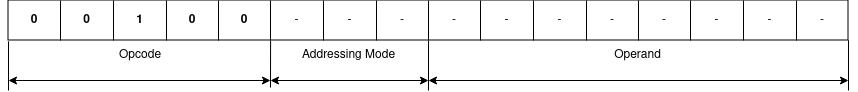
\includegraphics[scale=0.40]{img/Andromeda-NND.drawio}
    \end{center}


    \subsubsection{Example}
    \begin{verbatim}
            org(0x0000)
        def entry:
            lda.imm     0b00001101
            nnd.imm     0b00101110
            hlt
    \end{verbatim}
    \par The code above would result in $11110011_{2}$ being stored in the Accumulator.

\pagebreak
\subsection{Jump}\label{subsec:jmp}
    \subsubsection{Syntax}
    \begin{verbatim}jmp.[addressing mode]   [8-bit immediate]\end{verbatim}
    \subsubsection{Description}
    $PC \leftarrow OperandValue$
    \par Load the value indicated the operand value into the program counter.

    \subsubsection{Encoding}
    \begin{center}
        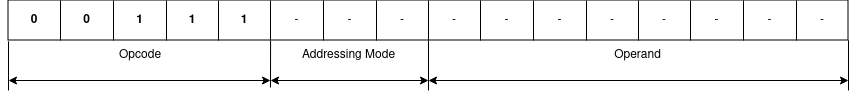
\includegraphics[scale=0.40]{img/Andromeda-JMP.drawio}
    \end{center}

    \subsubsection{Example}
    \begin{verbatim}
        org(0x0000)
    def entry:
        lda.imm     10
        jmp.off     0x03
        add.imm     1
        hlt
        add.imm     2
        hlt
    \end{verbatim}
    \par The code above would result in `12' in the Accumulator.
    The jump instruction would skip the `\texttt{add.imm 1}'  and  the first \texttt{hlt} instructions, by jumping to address $0004_{16}$.
    As a result, the `\texttt{add.imm 2}' instruction would be executed.

\pagebreak
\subsection{Jump to Subroutine}\label{subsec:jsr}
    \subsubsection{Syntax}
    \begin{verbatim}jsr.[addressing mode]   [8-bit immediate]\end{verbatim}
    \subsubsection{Description}
    $Accumulator \leftarrow PC + 1$; $PC \leftarrow OperandValue$
    \par Load a pointer to the next instruction into the Accumulator.
    Load the operand value into the program counter.
    \subsubsection{Encoding}
    \begin{center}
        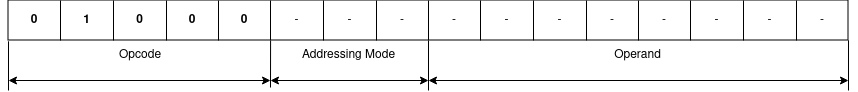
\includegraphics[scale=0.40]{img/Andromeda-JSR.drawio}
    \end{center}


\subsubsection{Example}
    \begin{verbatim}
        org(0x0000)
    def main:
        jsr.off     main.my_subroutine
        ; More instructions for main...
        hlt

    subdef my_subroutine:
        sta.dir     0x01
        ; Do subroutine stuff here
        jmp.dir     0x01
    \end{verbatim}
    \par The code above might show how a typical subroutine call might work.
    The \texttt{jsr.off} instruction stores a return address into the accumulator.
    The called subroutine, \texttt{my\_routine}, saves that return vector into $FF01_{16}$
    so that the subroutine can return to that address using a \texttt{jmp.dir} instruction.

\pagebreak
\subsection{Jump if the Accumulator is Not Signed}\label{subsec:jns}
    \subsubsection{Syntax}
    \begin{verbatim}jns.[addressing mode]   [8-bit immediate]\end{verbatim}
    \subsubsection{Description}
    $if\ (Accumulator \geq 0)\ \{ PC \leftarrow OperandValue \}$
    \par If the contents of the Accumulator are greater than, or equal to, zero, load the operand value into the PC\@.
    \subsubsection{Encoding}
    \begin{center}
        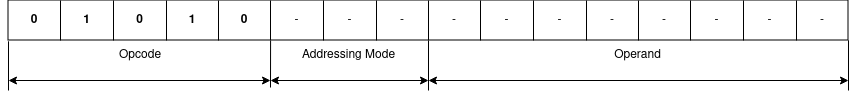
\includegraphics[scale=0.40]{img/Andromeda-JNS.drawio}
    \end{center}

    \subsubsection{Example}
    \begin{verbatim}
        org(0x0000)
    def entry:
        lda.imm     -2
        jns.off     greater_equal_to_zero
        lda.imm     1
        hlt
    def greater_equal_to_zero:
        lda.imm     2
        hlt
    \end{verbatim}
    \par The above code would result in a `1' loaded into the Accumulator.
    The \texttt{jns.off} instruction does not cause a jump because the Accumulator
    is greater than or equal to zero (eg it is not signed).

\pagebreak
\subsection{Jump if the Accumulator is Not Zero}\label{subsec:jnz}
    \subsubsection{Syntax}
    \begin{verbatim}jnz.[addressing mode]   [8-bit immediate]\end{verbatim}
    \subsubsection{Description}
    $if\ (Accumulator \neq 0)\ \{ PC \leftarrow OperandValue \}$
    \par If the contents of the Accumulator are not equal to zero, load the operand value into the PC\@.
    \subsubsection{Encoding}
    \begin{center}
        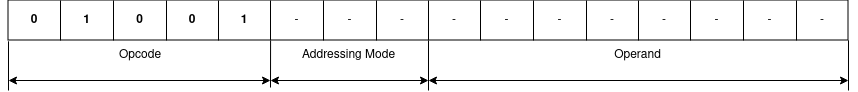
\includegraphics[scale=0.40]{img/Andromeda-JNZ.drawio}
    \end{center}

    \subsubsection{Example}
    \begin{verbatim}
        org(0x0000)
    def entry:
        lda.imm     -2
        jnz.imm     not_zero
        lda.imm     1
        hlt
    def not_zero:
        lda.imm     2
        hlt
    \end{verbatim}
    The above code would result in a `2' loaded into the Accumulator.
    A jump to the label \texttt{not\_zero} would occur because the Accumulator
    contains a non-zero value.

\pagebreak
\subsection{Halt}\label{subsec:halt}
    \subsubsection{Description}
    $HFF \leftarrow 1$
    \par Stop the system clock by setting the halt flip-flop.
    \subsubsection{Encoding}
    \begin{center}
        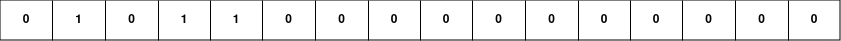
\includegraphics[scale=0.40]{img/Andromeda-HLT.drawio}
    \end{center}

\subsection{No Operation}\label{subsec:nop}
    \subsubsection{Description}
    $ -- $
    \par Continue to the next instruction without changing the machine's state.
    \subsubsection{Encoding}
    \begin{center}
        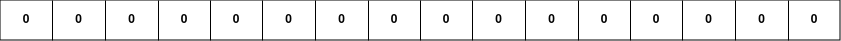
\includegraphics[scale=0.40]{img/Andromeda-NOP.drawio}
    \end{center}

\subsection{Reference Card}\label{subsec:reference-card2}